%% if some package prevents compilation, remove it

\documentclass[a4paper, 10pt]{article}
\usepackage{fullpage}
\usepackage{titling}
\usepackage{graphicx}
\usepackage{xcolor}
\usepackage{amsmath}
\usepackage{amssymb}
\usepackage{amsthm}
\usepackage{hyperref}
\usepackage{IEEEtrantools} 
\usepackage{bbm}
\usepackage{lineno}
\usepackage{multirow}
\usepackage{longtable}
\usepackage{makecell}
\usepackage{lipsum}
\usepackage{etoolbox} %% <- for \pretocmd and \apptocmd
\usepackage{algorithm}
\usepackage[noend]{algpseudocode}

\setlength{\droptitle}{-6em}   % This is your set screw, for shifting up the title
\renewcommand{\baselinestretch}{1.1}
\setlength{\parskip}{0.5em}

\author{Shivam and Sharan
  \\ September 2021}
\date{}
\title{FMA-PG Notes}

\makeatletter %% <- make @ usable in macro names
\newcommand*\linenomathpatch{\@ifstar{\linenomathpatch@AMS}{\linenomathpatch@}}
\newcommand*\linenomathpatch@[1]{
  \expandafter\pretocmd\csname #1\endcsname {\linenomathWithnumbers}{}{}
  \expandafter\pretocmd\csname #1*\endcsname{\linenomathWithnumbers}{}{}
  \expandafter\apptocmd\csname end#1\endcsname {\endlinenomath}{}{}
  \expandafter\apptocmd\csname end#1*\endcsname{\endlinenomath}{}{}
}
\newcommand*\linenomathpatch@AMS[1]{
  \expandafter\pretocmd\csname #1\endcsname {\linenomathWithnumbersAMS}{}{}
  \expandafter\pretocmd\csname #1*\endcsname{\linenomathWithnumbersAMS}{}{}
  \expandafter\apptocmd\csname end#1\endcsname {\endlinenomath}{}{}
  \expandafter\apptocmd\csname end#1*\endcsname{\endlinenomath}{}{}
}
\let\linenomathWithnumbersAMS\linenomathWithnumbers
\patchcmd\linenomathWithnumbersAMS{\advance\postdisplaypenalty\linenopenalty}{}{}{}
\makeatother %% revert @
\linenomathpatch{IEEEeqnarray}
\linenomathpatch{equation}
\linenomathpatch*{gather}
\linenomathpatch*{multline}
\linenomathpatch*{align}
\linenomathpatch*{alignat}
\linenomathpatch*{flalign}

\DeclareMathOperator{\E}{\mathbb{E}}

\begin{document}
\maketitle
\vspace{-2cm}
% \linenumbers

\section{Appendix}
\subsection{Experiments on the Tabular CliffWorld Environment}
In this section, we study the performance of five different policy gradient (PG) algorithms, sPPO (Softmax PPO\footnote{Note that this is NOT the sPPO of Section 6.2; we just overloaded this notation.}, FMA-PG with a softmax policy, see Eq. 8 in main text), MDPO, PPO, TRPO, and TRPO with KL regularization (which we call as TRPO-KL). We use a tabular gridworld environment called CliffWorld and a tabular softmax policy parameterization. The environment description and its properties are discussed in Figure \ref{fig: cliffworld}.

\begin{figure}[!hbp]
  \centering
  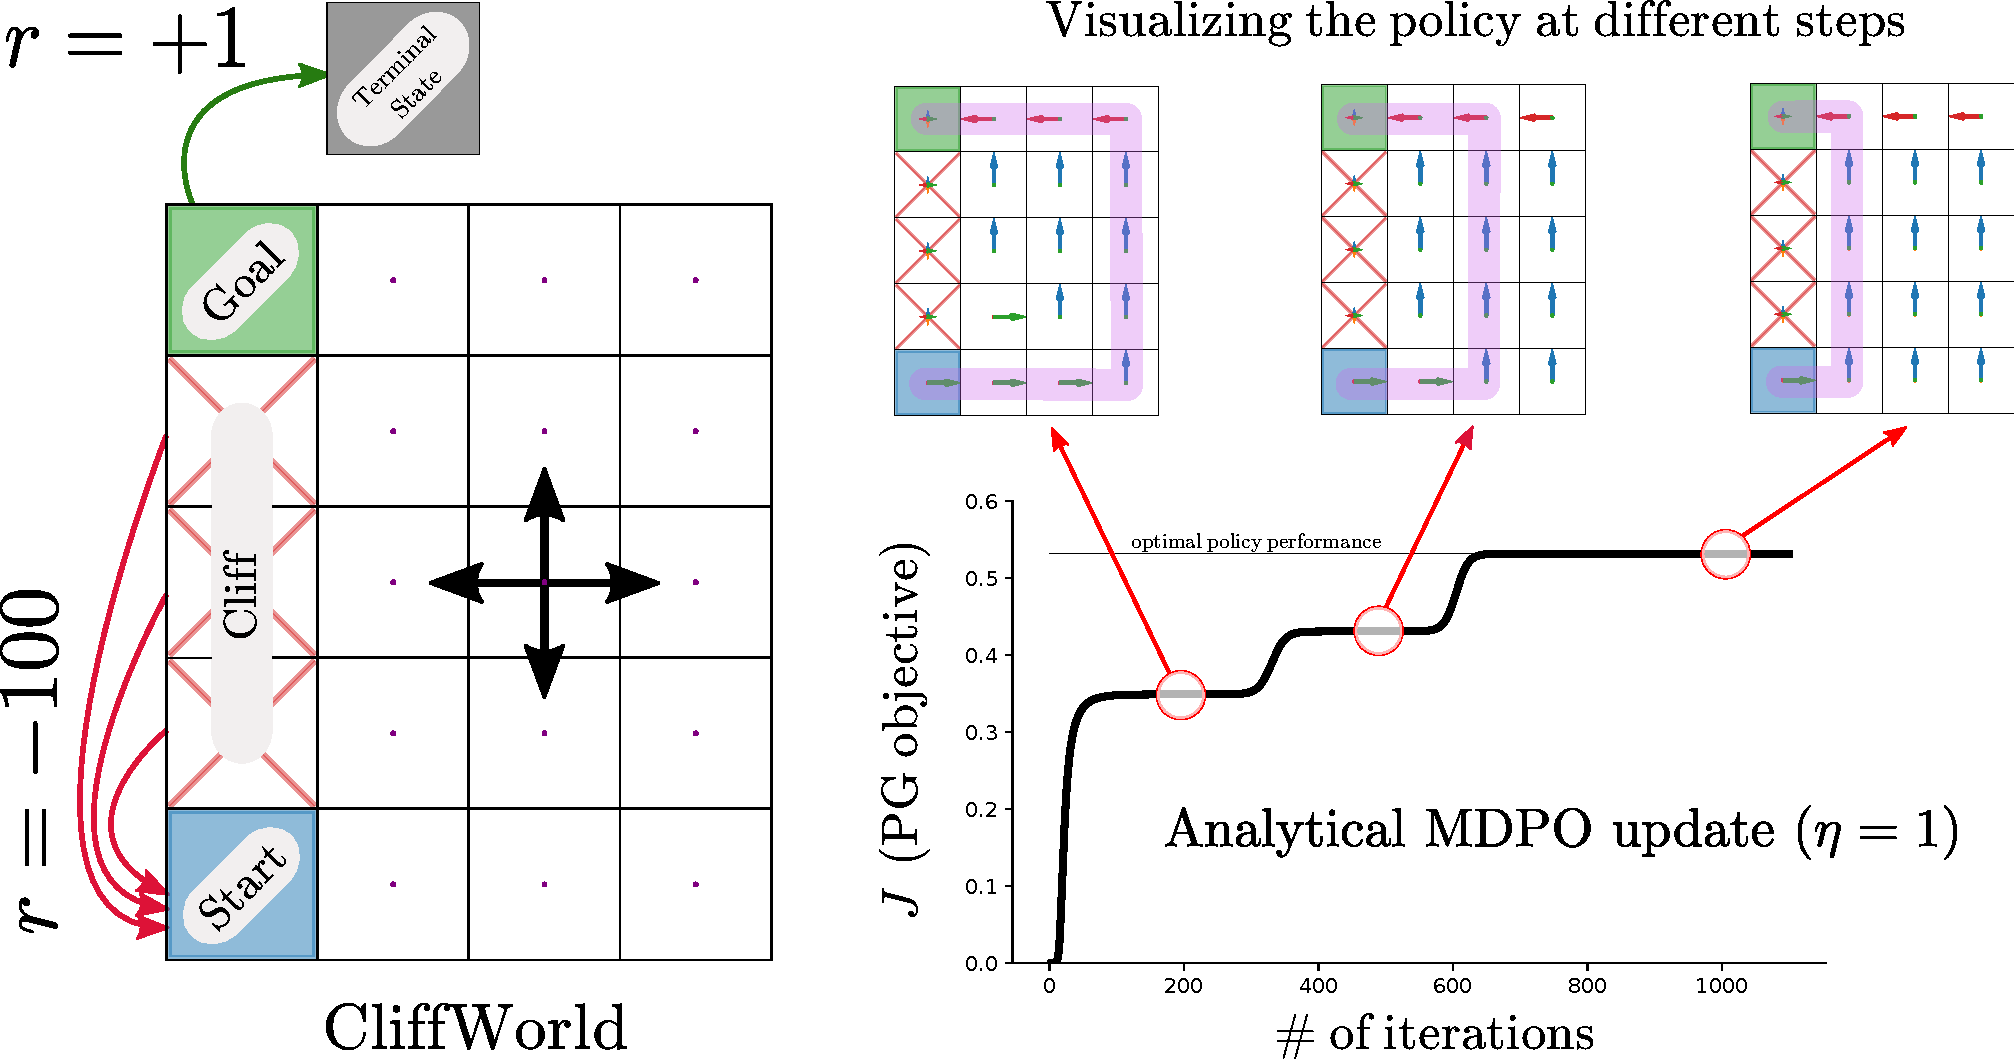
\includegraphics[scale=0.36]{tabular_figures/cliffworld.pdf}
  \caption{The episodic CliffWorld environment and the learning curve for MDPO on it illustrating three different locally optimal policies. \textbf{(Left)} We consider a variant of the CliffWorld environment (Example 6.6, Sutton and Barto, 2018) containing 21 different states and four actions per state. The agent starts in the \texttt{Start} state and has four cardinal actions which deterministically move it into the corresponding next state. The objective is to reach the \texttt{Goal} state as quickly as possible. If the agent falls into a state marked by \texttt{Cliff}, any subsequent action taken by it moves it back to the start state and yields a reward of $-100$. Similarly, once in the goal state, any action takes the agent into the terminal state and yields a reward of $+1$. All the other transitions have zero reward and the discount factor is $\gamma = 0.9$. It is easy to see that the optimal policy will have a value of $v^*(s_0) = 0 + \gamma \cdot 0 + \cdots + \gamma^5 \cdot 0 + \gamma^6 \cdot 1 = 0.9^6 = 0.53$. \textbf{(Right)} We show the learning curve for the analytical MDPO update using $\eta = 1$. This curve shows three different locally optimal policies. We later show in our experiments, that the different PG agents often get stuck on one of these policies.}
  \label{fig: cliffworld}
\end{figure}

To make the results easier to interpret and make them closely follow the theoretical properties of the PG methods, we assume full access to the environment dynamics and use the analytically calculated expected gradient updates for all the five algorithms. Doing so, essentially made this a study of the optimization properties of the above five PG algorithms. We trained each of the method for 2000 iterations. Each iteration consisted of one or multiple inner updates (we represent this number by $m$); these updates are performed in an off-policy fashion that is typical of all these algorithms (also see Algorithm 1, main paper). We also sweeped over the relevant parameters of the PG algorithms. For sPPO and MDPO, this was $\eta \in \{2^{-13}, 2^{-12}, \ldots, 2^3\}$ and inner loop stepsize $\alpha \in \{2^{-13}, 2^{-12}, \ldots, 2^3\}$. For PPO, we sweeped over the stepsize $\alpha \in \{2^{-13}, 2^{-12}, \ldots, 2^3\}$ and the clipping parameter $\epsilon \in \{0.1, 0.2, \ldots, 0.9\}$. For TRPO, we sweeped over the trust region size $\delta \in \{2^{-13}, 2^{-11}, \ldots, 2^{13}\}$ and the line search stepsize decay parameter $\text{df} \in \{0.1, 0.2, \ldots, 0.9\}$. And for TRPO-KL (see \S \ref{sec: trpo_kl}), this was KL regularization factor $\zeta \in \{2^{-13}, 2^{-11}, \ldots, 2^{13}\}$ and inner loop stepsize $\alpha \in \{2^{-13}, 2^{-12}, \ldots, 2^3\}$.

In the next section, we present the learning curves for these algorithms corresponding to the best hyperparameter configurations. After that we present the parameter sensitivity plots. We then describe our conclusions from these experiments. Finally, we also include the gradient calculations used in our implementations and associated details for all the methods.

\subsubsection{Learning Curves and Parameter Sensitivity Plots}
We show the performance of the five algorithms against the number of outer loop iterations in Figure \ref{fig: learning_curves}. The three different subplots correspond to a different number of inner updates\footnote{For TRPO, in the third subplot we just reused the performance from $m=100$. From our sensitivity plots (Figure \ref{fig: sensitivity}) we observed that the performance of TRPO saturated after $m = 10$; in particular the TRPO sensitivity plots are identical for $m=10$ and $m=100$. Therefore, its performance at $m=1000$ should be exactly equivalent to its performance at $m=100$ and consequently we skipped running that experiment.}. To select the hyperparameters for each setting, we ran sweeps over different configurations and chose the ones that resulted in the best final performance at the end of 2000 iterations.

From this figure, we see that TRPO learned the optimal policy in less than 20 iterations. Whereas, PPO got stuck in a ``safe'' sub-optimal policy. MDPO, sPPO, and TRPO-KL were all able to achieve the optimal policy with 100 and 1000 number of inner iterations, but got stuck in the suboptimal policy with 10 number of inner iterations. We further observe that increasing the number of inner loop iterations helped all the methods, except TRPO (which was already super fast), to improve the convergence speed. We should also mention, although TRPO had the faster convergence, its update was also the costliest (more than ten times slower than the rest of the methods) in terms of wall time. 

We show the complete parameter sweeps for the different methods in Figure \ref{fig: sensitivity}. The different rows correspond to different algorithms and the columns correspond to different number of inner loop updates. Each algorithm has two parameters: the $x$ axis gives the value of one of these parameters and the shaded curves correspond to the other parameter. The $y$ axis shows the final performance of the algorithm at the end of 2000 iterations corresponding to the particular parameter configuration. We also include the sensitivity plots for sPPO and MDPO under analytical updates, which is equivalent of doing an infinite number of inner loop updates ($m = \infty$) with a small enough stepsize $\alpha$.

From this figure we see that for $m=1$ all the algorithms, except TRPO, had a poor performance. And as the value of $m$ increased, these algorithms were able to perform well with a large number of stepsizes. We also note that, each of sPPO, MDPO, and TRPO-KL achieved the optimal policy for some parameter configurations, whereas PPO failed to achieve the optimal policy for any stepsize configuration we tried. sPPO, MDPO, and TRPO-KL had good performance for a range of parameters. Also, not the that for all values of $\eta < 1 - \gamma = 0.1$, which was suggested by the theory for sPPO, worked well. TRPO had a very low sensitivity for all its parameters, probably because TRPO uses the (near) optimal steepest ascent direction with the maximal stepsize, achieved via line search. This gives TRPO much better convergence properties, especially in this case where there are no sampling or estimation errors. Also, we think that the trust region parameter $\delta = 4$ was already too small for this problem and therefore TRPO performed well for all the values below it. Interestingly, TRPO-KL (which corresponds to an unconstrained optimization problem and doesn't use line search) did not enjoy these properties. TRPO-KL's performance for certain values of $\zeta$ was very similar to PPO; and for other values was superior to PPO. And it was slighltly less sensitive to the hyperparameters as compared to sPPO and MDPO.

\begin{figure}[!bp]
  \centering
  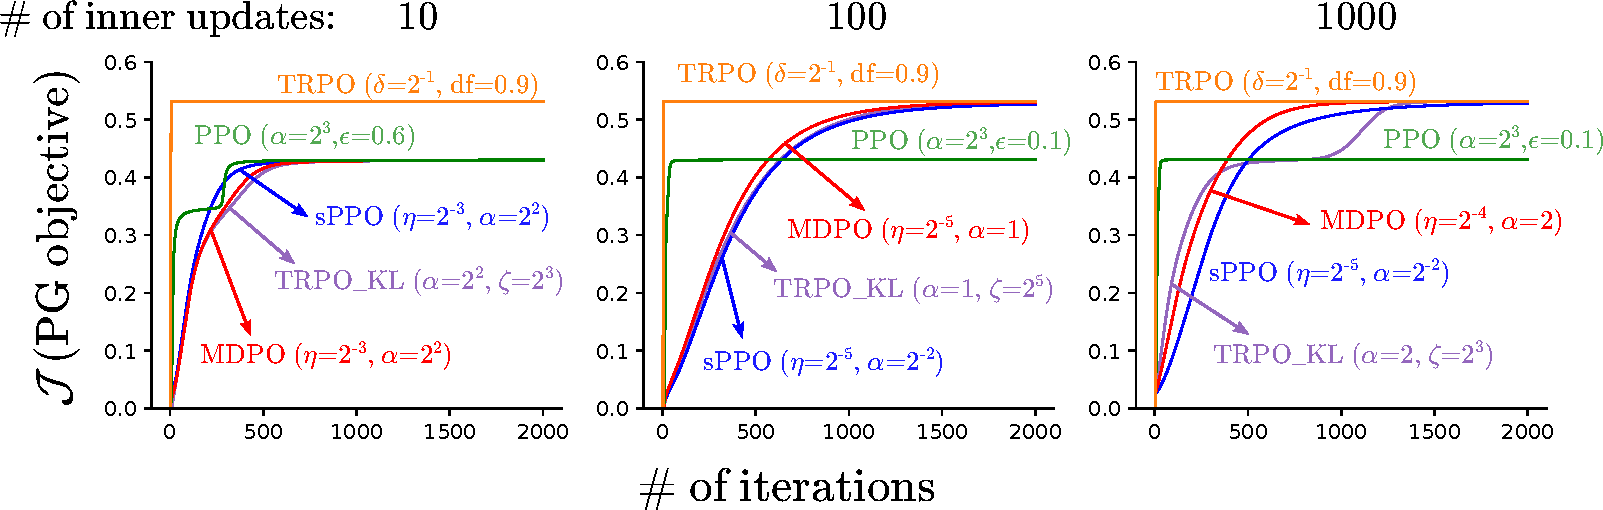
\includegraphics[scale=0.6]{tabular_figures/learning_curves.pdf}
  \caption{The learning curves for the five PG algorithms on the CliffWorld environment for different number of inner loop updates. All the updates were done using exact gradient calculations, i.e. there was no sampling involved.}
  \label{fig: learning_curves}
\end{figure}

\begin{figure}[!bp]
  \centering
  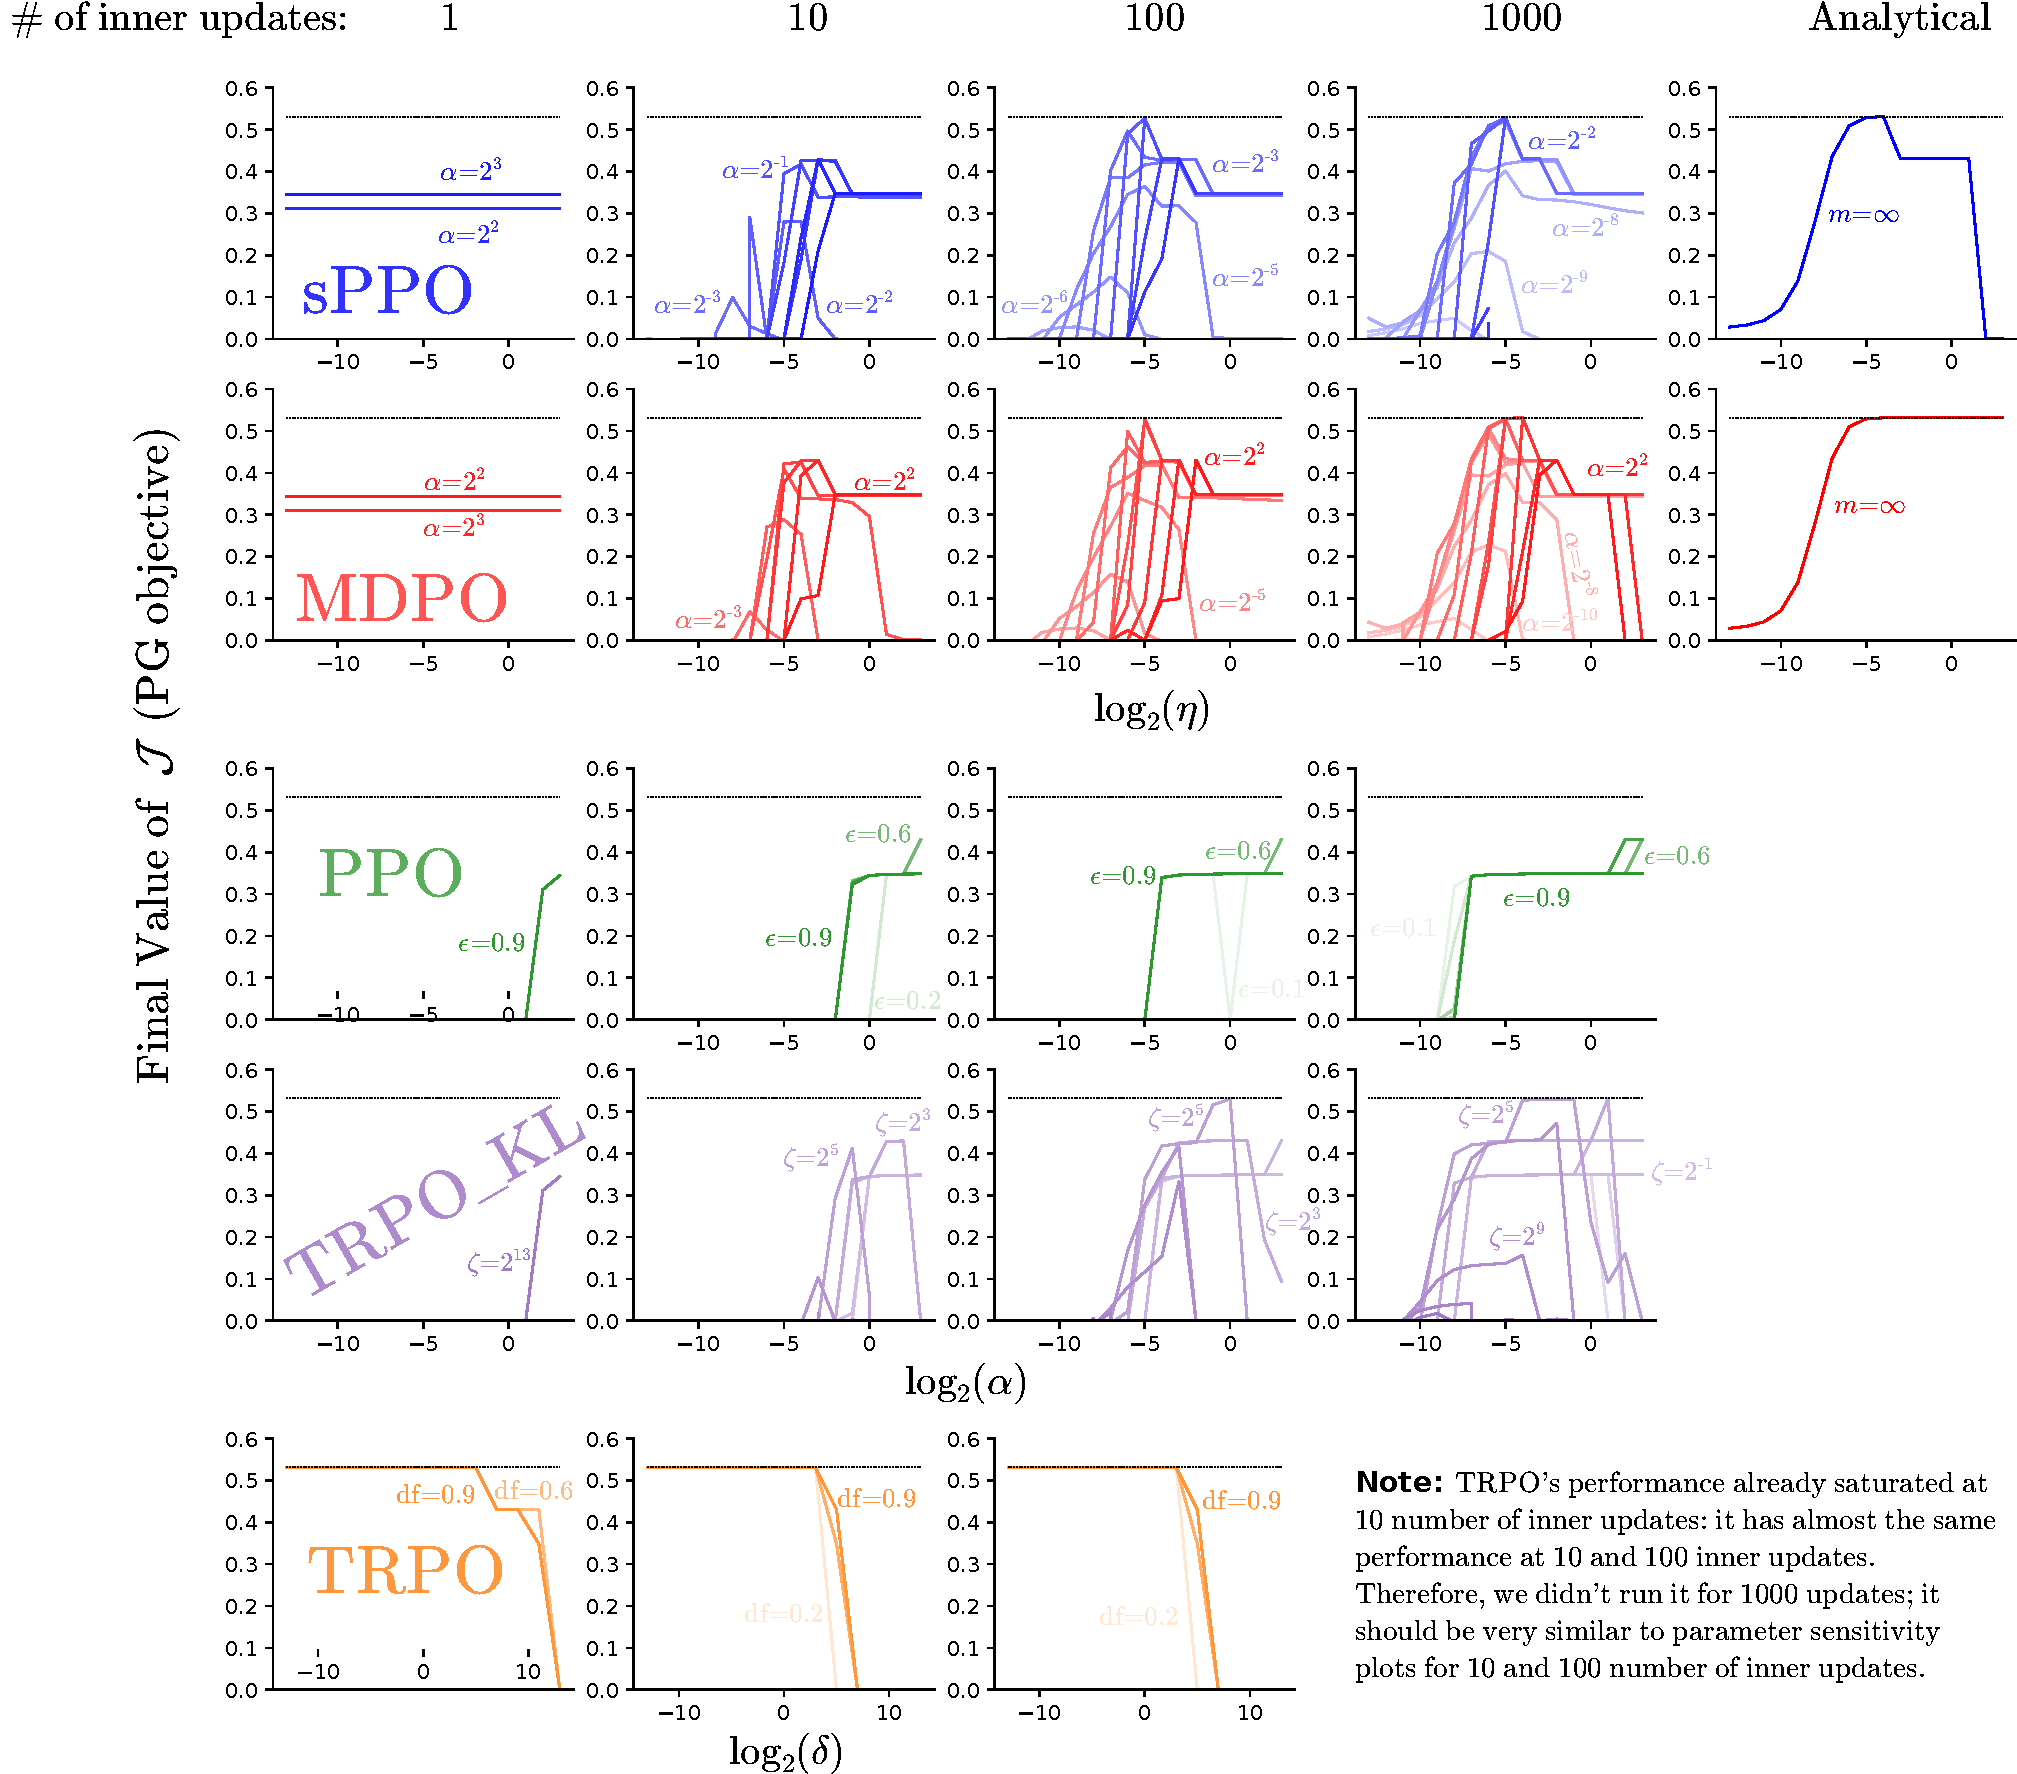
\includegraphics[scale=0.45]{tabular_figures/sensitivity.pdf}
  \caption{The parameter sensitivity plots for the five PG algorithms on the CliffWorld environment for different number of inner loop updates. The $x$ axis shows sweep over one parameter of the corresponding and the different color shaded curves correspond to another parameter. The faint black line near the top of each subplot depicts the value of the optimal policy.}
  \label{fig: sensitivity}
\end{figure}

\subsubsection{Conclusions}
The experiments for sPPO served as a verification of the theoretical properties of the FMA-PG framework studied in this paper. We also compared it against other popular policy gradient algorithms from a pure optimization perspective. Our results demonstrated that sPPO was competitive (or superior) to the popular PG methods. It was also somewhat robust to the hyperparameters; in particular we found that the algorithm, for all the value of $\eta$ suggested by theory, was able to converge to a locally optimal policy. The results also highlighted the importance of re-using data, i.e. doing multiple off-policy type of PG updates: as we increased the number of inner updates, the performance of all the methods seem to improve. They not only enjoyed faster convergence, but they also started to work for a wider range of parameters. This demonstrates the strength of these methods over simpler algorithms like REINFORCE (Williams, 1992) which only have a single update per batch of sampled data. To conclude, experiments with sPPO suggest that the FMA-PG framework is a systematic way of obtaining new policy gradient algorithms that enjoy desirable theoretical properties and can be competitive to existing PG method, as suggested by our empirical results. We also include the self-contained code for these experiments with the submission.

In the rest of this section, as promised, we give the calculations (the closed form analytical solutions for sPPO and MDPO, and the gradient expressions for all the five algorithms) employed in our empirical implementation.

\subsection{Softmax PPO with Tabular Parameterization}

\subsubsection{Closed Form Update with Direct Representation}
Our goal is to find the closed form solution to the following optimization problem (from Eq. 8, main paper):
\begin{equation}
  \pi_{t+1} = \arg\max_{\pi \in \Pi} \underbrace{\left[ \sum_s d^{\pi_t}(s) \sum_a p^{\pi_t}(a | s) \left(A^{\pi_t}(s, a) + \frac{1}{\eta} \right) \log \frac{p^\pi(s, a)}{p^{\pi_t}(s, a)} \right]}_{=: \ell^{\pi_t}_{\text{sPPO}}}, \label{eq: optim_problem_sppo}
\end{equation}
subject to the constraints on policy $p^\pi$. We will solve this problem by assuming the policy $\pi \equiv p^\pi$ as an $|\mathcal{S}| \times |\mathcal{A}|$ table satisfying the standard constraints
\begin{IEEEeqnarray*}{rCll}
  \sum_a p^\pi(a | s) &=& 1, & \quad \forall s \in \mathcal{S} \\
  p^\pi(a | s) &\geq& 0, & \quad \forall s \in \mathcal{S}, \; \forall a \in \mathcal{A}.
\end{IEEEeqnarray*}
We begin by formulating this problem using Lagrange multipliers $\{\lambda_s\}_{s \in \mathcal{S}}$ and $\{\lambda_{s, a}\}_{s, a \in \mathcal{S} \times \mathcal{A}}$ for all states $s$ and actions $a$:
\begin{IEEEeqnarray}{rCl}
  \mathcal{L}(p^\pi, \lambda_s, \lambda_{s, a}) &=& \sum_s d^{\pi_t}(s) \sum_a p^{\pi_t}(a | s) \left(A^{\pi_t}(s, a) + \frac{1}{\eta} \right) \log \frac{p^\pi(a | s)}{p^{\pi_t}(a | s)} \nonumber \\
  && - \sum_{s, a} \lambda_{s, a} p^\pi(a | s) - \sum_s \lambda_{s} \bigg( \sum_a p^\pi(a | s) - 1 \bigg),
\end{IEEEeqnarray}
where we abused the notation, in $\mathcal{L}(p^\pi, \lambda_s, \lambda_{s, a})$, by using $\lambda_s$ to represent the set $\{\lambda_s\}_{s \in \mathcal{S}}$ and $\lambda_{s, a}$ to represent the set $\{\lambda_{s, a}\}_{s, a \in \mathcal{S} \times \mathcal{A}}$. The KKT conditions (Theorem 12.1, Nocedal and Wright, 2006) for this constrained optimization problem can be written as:
\begin{align}
  \nabla_{p^\pi(b|x)} \mathcal{L}(p^\pi, \lambda_s, \lambda_{s, a}) &= 0, \quad \forall x \in \mathcal{S}, \; \forall b \in \mathcal{A} \tag{C1} \label{eq: KKT1} \\
  \sum_a p^\pi(a | s) &= 1, \quad \forall s \in \mathcal{S} \tag{C2} \label{eq: KKT2} \\
  p^\pi(a | s) &\geq 0, \quad \forall s \in \mathcal{S}, \; \forall a \in \mathcal{A} \tag{C3} \label{eq: KKT3} \\
  \lambda_s &\geq 0, \quad \forall s \in \mathcal{S} \tag{C4} \label{eq: KKT4} \\
  \lambda_{s} \bigg( \sum_a p^\pi(a | s) - 1 \bigg) &= 0, \quad \forall s \in \mathcal{S} \tag{C5} \label{eq: KKT5} \\
  \lambda_{s, a} p^\pi(a | s) &= 0, \quad \forall s \in \mathcal{S}, \; \forall a \in \mathcal{A}. \tag{C6} \label{eq: KKT6}
\end{align}

We now solve this system. Simplifying Eq. \ref{eq: KKT1} for an arbitrary state-action pair $(x, b)$ gives us:
\begin{IEEEeqnarray}{lrCl}
  & \nabla_{p^\pi(b | x)} \mathcal{L}(p^\pi, \lambda_s, \lambda_{s, a}) &=& d^{\pi_t}(x) p^{\pi_t}(b|x) \left( A^{\pi_t}(x, b) + \frac{1}{\eta} \right) \frac{1}{p^\pi(b|x)} - \lambda_{x, b} - \lambda_x = 0 \nonumber \\
  \Rightarrow & p^\pi(b | x) &=& \frac{d^{\pi_t}(x) p^{\pi_t}(b|x) (1 + \eta A^{\pi_t}(x, b))}{\eta (\lambda_x + \lambda_{x, b})}. \label{eq: lagrangian_derivative_sppo}
\end{IEEEeqnarray}
Let us set 
\begin{equation}
  \lambda_{s, a} = 0, \quad \forall s \in \mathcal{S}, \; \forall a \in \mathcal{A}.
\end{equation}
Combining Eq. \ref{eq: lagrangian_derivative_sppo} with the second KKT condition gives us
\begin{equation}
  \lambda_s = \frac{1}{\eta} \sum_a d^{\pi_t}(s) p^{\pi_t}(a|s) (1 + \eta A^{\pi_t}(s, a)).
\end{equation}
Therefore, with the standard coverage assumption $d^{\pi_t}(s) > 0$, $p^\pi(a | s)$ becomes
\begin{equation}
  p^\pi(a | s) = \frac{p^{\pi_t}(a|s) (1 + \eta A^{\pi_t}(s, a))}{\sum_b p^{\pi_t}(b|s) (1 + \eta A^{\pi_t}(s, b))}.
\end{equation}
Note that $d^{\pi_t}(s), p^{\pi_t}(a|s) \geq 0$ for any state-action pair, since they are proper measures. We also need to ensure that
\begin{equation*}
  1 + \eta A^{\pi_t}(s, a) \geq 0
\end{equation*}
to satisfy the third and fourth KKT conditions. One straightforward way to achieve this is to define $p^\pi(a | s) = 0$ whenever $1 + \eta A^{\pi_t}(s, a) < 0$, and accordingly re-define $\lambda_s$. This gives us the final solution to our original optimization problem (Eq. \ref{eq: optim_problem_sppo}):
\begin{equation}
  \pi_{t+1} = p^\pi(s, a) = \frac{p^{\pi_t}(a|s) \max(1 + \eta A^{\pi_t}(s, a), 0)}{\sum_b p^{\pi_t}(b|s) \max(1 + \eta A^{\pi_t}(s, b), 0)}.
\end{equation}
However, it leaves us one last problem to deal with: Is it always true that given any state $s$, there always exists atleast one action $a$, such that $1 + \eta A^{\pi_t}(s, a) \geq 0$? Because otherwise, we would fail to satisfy the second KKT condition. But not that this is not a problem since we can put a condition on $\eta$ in order to fulfill this constraint.

\subsubsection{Gradient of the Loss Function with Softmax Policy Representation}
Consider the softmax policy representation
\begin{equation}
  p^\pi(b | x) = \frac{e^{\theta(x, b)}}{\sum_c e^{\theta(x, c)}}, \label{eq: softmax}
\end{equation}
where $\theta(x, b)$ for all state-action pairs $(x, b)$ are action preferences maintained in a table (tabular parameterization). Also note that the derivative of the policy with respect to the action preferences is given by
\begin{equation}
  \frac{\partial}{\partial \theta(s, a)} p^\pi(b | x) = \mathbb{I}(x = s) \Big( \mathbb{I}(b = a) - p^\pi(a | x) \Big) p^\pi(b | x),
\end{equation}
where $\mathbb{I}(a = b)$ is the identity function when $a = b$ and zero otherwise. 
We will use gradient ascent to approximately solve Eq. \ref{eq: optim_problem_sppo}; to do that, the quantity of interest is
\begin{align}
  \frac{\partial}{\partial \theta(s, a)} \ell^{\pi_t}_{\text{sPPO}} &= \sum_{x \in \mathcal{S}} \sum_{b \in \mathcal{A}} \left[ \frac{\partial}{\partial \theta(s, a)} p^\pi(b | x) \right] \left[ \frac{\partial}{\partial p^\pi(b | x)} \ell^{\pi_t}_{\text{sPPO}} \right] \tag*{(using total derivative)} \\
  &= \sum_{x, b} \Big[ \mathbb{I}(x = s) \Big( \mathbb{I}(b = a) - p^\pi(a | x) \Big) p^\pi(b | x) \Big] \left[ d^{\pi_t}(x) p^{\pi_t}(b|x) \left( A^{\pi_t}(x, b) + \frac{1}{\eta} \right) \frac{1}{p^\pi(b|x)} \right] \nonumber \\
  &= \E_{X \sim d^{\pi_t}, B \sim p^{\pi_t}(\cdot | X)} \left[ \mathbb{I}(X = s) \Big( \mathbb{I}(B = a) - p^\pi(a | x) \Big) \left( A^{\pi_t}(X, B) + \frac{1}{\eta} \right) \right] \\
  &= d^{\pi_t}(s) \sum_b \Big( \mathbb{I}(b = a) - p^\pi(a | s) \Big) p^{\pi_t}(b|s) \left( A^{\pi_t}(s, b) + \frac{1}{\eta} \right) \nonumber \\
  &= d^{\pi_t}(s) \left[ p^{\pi_t}(a|s) \left( A^{\pi_t}(s, a) + \frac{1}{\eta} \right) - p^\pi(a | s) \sum_b p^{\pi_t}(b|s) \left(A^{\pi_t}(s, b) + \frac{1}{\eta} \right) \right] \nonumber \\
  &= d^{\pi_t}(s) \left[ p^{\pi_t}(a|s) \left( A^{\pi_t}(s, a) + \frac{1}{\eta} \right) - \frac{p^\pi(a | s)}{\eta} \right], \nonumber
\end{align}
Now we can simply update the inner loop of FMA-PG (Algorithm 1, main paper) via gradient ascent:
\begin{equation}
  \theta(s, a) \; \leftarrow \; \theta(s, a) + \alpha d^{\pi_t}(s) \left[ p^{\pi_t}(a|s) \left( A^{\pi_t}(s, a) + \frac{1}{\eta} \right) - \frac{p^\pi(a | s)}{\eta} \right].
\end{equation}

\subsection{Mirror Descent Policy Optimization (MDPO)}
In this section, we study the MDPO type FMA-PG update (Eq. 6). We first calculate the analytical solution to that optimization problem, and then calculate its gradient which we use in the experiments. However, in the analysis that follows, we we replace the advantage function $A^{\pi_t}$ with the action-value function $Q^{\pi_t}$ to make it same as the MDPO (Tomar et al., 2020) update.
\subsubsection{Closed Form Update with Direct Parameterization}
While giving the MDPO type FMA-PG equation (Eq. 6), the paper considers the direct representation along with tabular parameterization of the policy, albeit with a small change in notation as compared to the previous subsection: $\pi(a|s) \equiv p^\pi(a|s, \theta)$. However, since this notation is more cumbersome, we will stick with our the notation of the previous subsection: $\pi(a|s) \equiv p^\pi(a|s)$. The constraints on the parameters $p^\pi(s, a)$ are the same as before: $\sum_a p^\pi(a | s) = 1, \; \forall s \in \mathcal{S}$; and $p^\pi(a | s) \geq 0, \; \forall s \in \mathcal{S}, \; \forall a \in \mathcal{A}$. Our goal, this time, is to solve the following optimization problem (from Eq. 6, main paper)
\begin{equation}
  \pi_{t+1} = \arg\max_{\pi \in \Pi} \underbrace{\left[ \sum_s d^{\pi_t}(s) \sum_a p^{\pi_t}(a|s) \left( Q^{\pi_t}(s, a) \frac{p^\pi(a | s)}{p^{\pi_t}(a | s)} - \frac{1}{\eta} D_\phi (p^\pi(\cdot | s), p^{\pi_t}(\cdot | s)) \right) \right]}_{=: \ell^{\pi_t}_{\text{MDPO}}}, \label{eq: optim_problem_mdpo}
\end{equation}
with the mirror map as the negative entropy (Eq. 5.27, Beck and Teboulle, 2002). This particular choice of the mirror map simplifies the Bregman divergence as follows
\begin{equation}
  D_\phi (p^\pi(\cdot | s), p^{\pi_t}(\cdot | s)) = \text{KL}(p^\pi(\cdot | s) \| p^{\pi_t}(\cdot | s)) := \sum_a p^\pi(a | s) \log \frac{p^\pi(a | s)}{p^{\pi_t}(a | s)}.
\end{equation}
The optimization problem (Eq. \ref{eq: optim_problem_mdpo}) then simplifies to
\begin{equation}
  \pi_{t+1} = \arg\max_{\pi \in \Pi} \left[ \sum_s d^{\pi_t}(s) \sum_a p^{\pi_t}(a|s) \left( Q^{\pi_t}(s, a) \frac{p^\pi(a | s)}{p^{\pi_t}(a | s)} - \frac{1}{\eta} \sum_{a'} p^\pi(a' | s) \log \frac{p^\pi(a' | s)}{p^{\pi_t}(a' | s)} \right) \right].
\end{equation}

Proceeding analogously to the previous subsection, we use Lagrange multipliers $\lambda_s$, $\lambda_{s, a}$ for all states $s$ and actions $a$ to obtain the function
\begin{IEEEeqnarray}{rCl}
  \mathcal{L}(p^\pi, \lambda_s, \lambda_{s, a}) &=& \sum_s d^{\pi_t}(s) \sum_a p^{\pi_t}(a|s) Q^{\pi_t}(s, a) \frac{p^\pi(a | s)}{p^{\pi_t}(a | s)} - \frac{1}{\eta} \sum_s d^{\pi_t}(s) \sum_{a'} p^\pi(a' | s) \log \frac{p^\pi(a' | s)}{p^{\pi_t}(a' | s)} \nonumber \\
  && - \sum_{s, a} \lambda_{s, a} p^\pi(a | s) - \sum_s \lambda_{s} \bigg( \sum_a p^\pi(a | s) - 1 \bigg).
\end{IEEEeqnarray}
The KKT conditions are exactly the same as before (Eq. \ref{eq: KKT1} to Eq. \ref{eq: KKT6}).

Again, we begin by solving the first KKT condition:
\begin{IEEEeqnarray}{lrCl}
  & \nabla_{p^\pi(b | x)} \mathcal{L}(p^\pi, \lambda_s, \lambda_{s, a}) &=& d^{\pi_t}(x) p^{\pi_t}(b|x) \frac{Q^{\pi_t}(x, b)}{p^{\pi_t}(b | x)} - \frac{d^{\pi_t}(x)}{\eta} \left[ \log \frac{p^\pi(b | x)}{p^{\pi_t}(b | x)} + 1 \right] - \lambda_{x, b} - \lambda_x \nonumber \\
  &&=& \frac{d^{\pi_t}(x)}{\eta} \left[ \eta Q^{\pi_t}(x, b) - \log \frac{p^\pi(b | x)}{p^{\pi_t}(b | x)} - 1 - \frac{\eta (\lambda_{x, b} + \lambda_x)}{d^{\pi_t}(x)} \right] \nonumber \\
  &&=& 0 \nonumber \\
  \Rightarrow & \log \frac{p^\pi(b | x)}{p^{\pi_t}(b | x)} &=& \eta Q^{\pi_t}(x, b) - \frac{\eta (\lambda_{x, b} + \lambda_x)}{d^{\pi_t}(x)} - 1 \nonumber \\
  \Rightarrow & p^\pi(b | x) &=& p^{\pi_t}(b | x) \cdot e^{\eta Q^{\pi_t}(x, b)} \cdot e^{- \frac{\eta (\lambda_{x, b} + \lambda_x)}{d^{\pi_t}(x)} - 1}, \label{eq: lagrangian_derivative_mdpo}
\end{IEEEeqnarray}
where in the fourth line, we used the assumption that $d^{\pi_t}(x) > 0$ for all states $x$. We again set
\begin{equation}
  \lambda_{s, a} = 0, \quad \forall s \in \mathcal{S}, \; \forall a \in \mathcal{A}.
\end{equation}
And, we put Eq. \ref{eq: lagrangian_derivative_mdpo} in the second KKT condition to get
\begin{equation}
  e^{- \frac{\eta \lambda_x}{d^{\pi_t}(x)} - 1} = \left( \sum_b p^{\pi_t}(b | x) \cdot e^{\eta Q^{\pi_t}(x, b)} \right)^{-1}.
\end{equation}
Therefore, we obtain
\begin{equation}
  p^\pi(a | s) = \frac{p^{\pi_t}(a | s) \cdot e^{\eta Q^{\pi_t}(s, a)}}{\sum_b p^{\pi_t}(b | s) \cdot e^{\eta Q^{\pi_t}(s, b)}}.
\end{equation}
This leaves one last problem: Can we ensure that $\lambda_s \geq 0$ for all states $s$? If not, then the fourth KKT condition cannot be satisfied. Again, we can set the stepsize $\eta$ in such a way, such that this constraint is always fulfilled.

\subsubsection{Gradient of the MDPO Loss Function with Tabular Softmax Representation}
We again take the softmax policy representation given by Eq. \ref{eq: softmax}, and compute $\nabla_{\theta(s, a)} \ell^{\pi_t}_{\text{MDPO}}$ for the MDPO loss (we substitute $Q^{\pi_t}$ with $A^{\pi_t}$ in this calculation):
\begin{align}
  \frac{\partial}{\partial \theta(s, a)} \ell^{\pi_t}_{\text{MDPO}} &= \sum_{x, b} \left[ \frac{\partial}{\partial \theta(s, a)} p^\pi(b | x) \right] \left[ \frac{\partial}{\partial p^\pi(b | x)} \ell^{\pi_t} \right] \tag*{(using total derivative)} \\
  &= \sum_{x, b} \Big[ \mathbb{I}(x = s) \Big( \mathbb{I}(b = a) - p^\pi(a | x) \Big) p^\pi(b | x) \Big] \left[ \frac{d^{\pi_t}(x)}{\eta} \left( \eta A^{\pi_t}(x, b) - \log \frac{p^\pi(b | x)}{p^{\pi_t}(b | x)} - 1 \right) \right] \nonumber \\
  &= \frac{d^{\pi_t}(s)}{\eta} \sum_b \Big( \mathbb{I}(b = a) - p^\pi(a | s) \Big) p^\pi(b | s) \left[ \eta A^{\pi_t}(s, b) - \log \frac{p^\pi(b | s)}{p^{\pi_t}(b | s)} - 1 \right] \nonumber \\
  &= \frac{d^{\pi_t}(s)}{\eta} p^\pi(a | s) \left[ \eta A^{\pi_t}(s, a) - \eta \sum_b p^\pi(b|s) A^{\pi_t}(s, b) - \log \frac{p^\pi(a | s)}{p^{\pi_t}(a | s)} + \text{KL}(p^\pi(\cdot | s) \| p^{\pi_t}(\cdot | s)) \right], \nonumber
\end{align}
where in the last line, we used the fact that
\begin{equation*}
  \sum_b p^\pi(b | s) \left[ \eta A^{\pi_t}(s, b) - \log \frac{p^\pi(b | s)}{p^{\pi_t}(b | s)} - 1 \right] = \eta \sum_b p^\pi(b|s) A^{\pi_t}(s, b) - \text{KL}(p^\pi(\cdot | s) \| p^{\pi_t}(\cdot | s)) - 1.
\end{equation*}

\subsection{Trust Region Policy Optimization (TRPO)}
At each step of the policy update, TRPO (Eq. 14, Schulman et al., 2015) solves the following problem:
\begin{equation}
  \max_\theta \; \underbrace{\sum_s d^{\pi_t}(s) \sum_a p^{\pi_\theta}(a | s) Q^{\pi_t}(s, a)}_{=: \mathcal{J}_{\text{TRPO}}} \qquad \text{subject to } \underbrace{\sum_s d^{\pi_t}(s) \cdot \text{KL}(p^{\pi_t}(\cdot | s) \| p^{\pi_\theta}(\cdot | s))}_{=: \mathcal{C}_{\text{TRPO}}} \leq \delta.  
\end{equation}
Unlike the sPPO and the MDPO updates, an analytical solution cannot be derived for this update (since it would require solving a system of non-trivial non-linear equations; to see this, try writing the KKT conditions for the above constrained optimization problem). Therefore, we will use gradient based methods to approximately solve this problem. From Appendix C of Schulman et al. (2015), the descent direction is given by $s \approx A^{-1} g$ where the vector $g$ is defined as $g_{(s, a)} := \frac{\partial}{\partial \theta(s, a)} \mathcal{J}_{\text{TRPO}}$, and the matrix $A$ is defined as $A_{(s, a), (s', a')} := \frac{\partial}{\partial \theta(s, a)} \frac{\partial}{\partial \theta(s', a')} \mathcal{C}_{\text{TRPO}}$. We analytically compute the expression for this direction assuming a softmax policy (Eq. \ref{eq: softmax}). The vector $g$ can be readily calculated as
\begin{align}
  \frac{\partial}{\partial \theta(s, a)} \mathcal{J}_{\text{TRPO}} &= \sum_x d^{\pi_t}(x) \sum_b Q^{\pi_t}(x, b) \frac{\partial p^{\pi_\theta}(b | x)}{\partial \theta(s, a)} \nonumber \\
  &= \sum_x d^{\pi_t}(x) \sum_b Q^{\pi_t}(x, b) \mathbb{I}(x = s) \Big( \mathbb{I}(b = a) - p^{\pi_\theta}(a | x) \Big) p^{\pi_\theta}(b | x) \nonumber \\
  &= \sum_x d^{\pi_t}(x) \mathbb{I}(x = s) \left[ \sum_b \mathbb{I}(b = a) p^{\pi_\theta}(b | x) Q^{\pi_t}(x, b) - p^{\pi_\theta}(a | x) \sum_b p^{\pi_\theta}(b | x) Q^{\pi_t}(x, b) \right] \nonumber \\
  &= d^{\pi_t}(s) p^{\pi_\theta}(a | s) \left[ Q^{\pi_t}(s, a) - \sum_b p^{\pi_\theta}(b | s) Q^{\pi_t}(s, b) \right]. \label{eq: trpo_gradient}
\end{align}
For calculating the matrix $A$, note that
\begin{equation*}
  \frac{\partial \mathcal{C}_{\text{TRPO}}}{\partial p^{\pi_\theta}(b | x)} = \frac{\partial}{\partial p^{\pi_\theta}(b | x)} \sum_s d^{\pi_t}(s) \sum_a p^{\pi_t}(a | s) \log \frac{p^{\pi_t}(a | s)}{p^{\pi_\theta}(a | s)} = - d^{\pi_t}(x) \frac{p^{\pi_t}(b | x)}{p^{\pi_\theta}(b | x)}.
\end{equation*}
Then using the law of total derivative gives us
\begin{align}
  \frac{\partial}{\partial \theta(s, a)} \mathcal{C}_{\text{TRPO}} &= \sum_{x, b} \frac{\partial p^{\pi_\theta}(b | x)}{\partial \theta(s, a)} \cdot \frac{\partial \mathcal{C}_{\text{TRPO}}}{\partial p^{\pi_\theta}(b | x)} \nonumber \\
  &= - \sum_{x, b} \mathbb{I}(x = s) \Big( \mathbb{I}(b = a) - p^{\pi_\theta}(a | x) \Big) p^{\pi_\theta}(b | x) \cdot d^{\pi_t}(x) \frac{p^{\pi_t}(b | x)}{p^{\pi_\theta}(b | x)} \nonumber \\
  &= - d^{\pi_t}(s) \sum_b \Big( \mathbb{I}(b = a) - p^{\pi_\theta}(a | s) \Big) p^{\pi_t}(b | s) \nonumber \\
  &= - d^{\pi_t}(s) \left[ \sum_b \mathbb{I}(b = a) p^{\pi_t}(b | s) - p^{\pi_\theta}(a | s) \sum_b p^{\pi_t}(b | s) \right] \nonumber \\
  &= - d^{\pi_t}(s) \Big[ p^{\pi_\theta}(a | s) - p^{\pi_t}(a | s) \Big]. \label{eq: trpo_kl_mid}
\end{align}
Finally, using the above result yields
\begin{IEEEeqnarray}{lrCl}
  & \frac{\partial}{\partial \theta(s, a)} \frac{\partial}{\partial \theta(s', a')} \mathcal{C}_{\text{TRPO}} &=& \frac{\partial}{\partial \theta(s, a)} d^{\pi_t}(s') \Big[ p^{\pi_\theta}(a | s) - p^{\pi_t}(a | s) \Big] \nonumber \\
  &&=& d^{\pi_t}(s') \cdot \frac{\partial}{\partial \theta(s, a)} p^{\pi_\theta}(a' | s') \nonumber \\
  &&=& \mathbb{I}(s'=s) \cdot d^{\pi_t}(s') \Big( \mathbb{I}(a'=a) - p^{\pi_\theta}(a | s') \Big) p^{\pi_\theta}(a' | s') \\
  \Rightarrow \quad & A_{(s, :), (s, :)} &=& d^{\pi_t}(s) \Big( \text{diag} (p^{\pi_\theta}(\cdot | s)) - p^{\pi_\theta}(\cdot | s) p^{\pi_\theta}(\cdot | s)^\top \Big),
\end{IEEEeqnarray}
where $p^{\pi_\theta}(\cdot | s) \in \mathbb{R}^{|\mathcal{A}|}$ is the vector defined as $[p^{\pi_\theta}(\cdot | s)]_a = p^{\pi_\theta}(a | s)$ and $A_{(s, :), (s, :)}$ denotes the square sub-block of the matrix $A$ corresponding to the given state $s$ and all the actions. In our experiments, since our $A$ matrix is small, we directly take its inverse to compute the update direction, thereby bypassing the conjugate method. Once we have the update direction, we then compute the maximal stepsize $\beta$ and perform an exponential backtracking line search as explained in the TRPO paper.

\subsection{TRPO with KL Regularization} \label{sec: trpo_kl}
We also study a variant of TRPO where instead of satisfying the KL constraint on the policy, we subtract it as a regularization term (we subtract because this is a maximization problem). The resulting optimization problem becomes:
\begin{equation}
  \max_\theta \; \underbrace{\left[ \sum_s d^{\pi_t}(s) \sum_a p^{\pi_\theta}(a | s) Q^{\pi_t}(s, a) - \zeta \sum_s d^{\pi_t}(s) \cdot \text{KL}(p^{\pi_t}(\cdot | s) \| p^{\pi_\theta}(\cdot | s)) \right]}_{=: \mathcal{J}_{\text{TRPO-KL}} = \mathcal{J}_{\text{TRPO}} - \zeta \mathcal{C}_{\text{TRPO}}}.  
\end{equation}
Note that this objective is almost the same as PPO with KL penalty (Eq. 8, Schulman et al., 2017) except that PPO uses the advantage function and we used the action value function. It is also similar to the objective stated in the TRPO paper (Section 4, Schulman et al., 2015) except that it has an average KL divergence instead of the max KL divergence. We can reuse Eq. \ref{eq: trpo_gradient} and Eq. \ref{eq: trpo_kl_mid} to compute its gradient:
\begin{align}
  \frac{\partial \mathcal{J}_{\text{TRPO-KL}}}{\partial \theta(s, a)} &= d^{\pi_t}(s) p^{\pi_\theta}(a | s) \left[ Q^{\pi_t}(s, a) - \sum_b p^{\pi_\theta}(b | s) Q^{\pi_t}(s, b) \right] + \zeta d^{\pi_t}(s) \Big[ p^{\pi_\theta}(a | s) - p^{\pi_t}(a | s) \Big].
\end{align}

\subsection{Proximal Policy Optimization (PPO)}
The Proximal Policy Optimization algorithm (Schulman et al., 2017) solves the following optimization problem at each iteration step:
\begin{equation}
  \max_\theta \; \underbrace{\sum_s d^{\pi_t}(s) \sum_a p^{\pi_t}(a | s) \cdot \min \left( \begin{matrix} \frac{p^{\pi_\theta}(a | s)}{p^{\pi_t}(a | s)} A^{\pi_t}(s, a), \\ \text{clip} \left[\frac{p^{\pi_\theta}(a | s)}{p^{\pi_t}(a | s)}, 1 - \epsilon, 1 + \epsilon \right] A^{\pi_t}(s, a) \end{matrix} \right)}_{=: \mathcal{J}_{\text{PPO}}}.
\end{equation}
The gradient of the objective $\mathcal{J}_{\text{PPO}}$ can be shown to be equivalent to
\begin{equation}
  \nabla \mathcal{J}_{\text{PPO}} = \sum_s d^{\pi_t}(s) \sum_a p^{\pi_t}(a | s) \cdot \mathbb{I} \Big( \text{cond}(s, a) \Big) \frac{\nabla p^{\pi_\theta}(a | s)}{p^{\pi_t}(a | s)} A^{\pi_t}(s, a),
\end{equation}
where 
\begin{equation}
  \text{cond}(s, a) = \left( A^{\pi_t}(s, a) > 0 \;\bigwedge\; \frac{p^{\pi_\theta}(a | s)}{p^{\pi_t}(a | s)} < 1 + \epsilon \right) \;\bigvee\; \left( A^{\pi_t}(s, a) < 0 \;\bigwedge\; \frac{p^{\pi_\theta}(a | s)}{p^{\pi_t}(a | s)} > 1 - \epsilon \right).
\end{equation}
Repeating our usual drill, we assume a softmax policy to obtain:
\begin{align}
  & \frac{\partial}{\partial \theta(s, a)} \mathcal{J}_{\text{PPO}} \nonumber \\
  &= \sum_x d^{\pi_t}(x) \sum_b \mathbb{I} \Big( \text{cond}(x, b) \Big) \frac{\partial p^{\pi_\theta}(b | x)}{\partial \theta(s, a)} A^{\pi_t}(x, b) \nonumber \\
  &= \sum_x d^{\pi_t}(x) \sum_b \mathbb{I} \Big( \text{cond}(x, b) \Big) \mathbb{I}(x = s) \Big( \mathbb{I}(b = a) - p^{\pi_\theta}(a | x) \Big) p^{\pi_\theta}(b | x) A^{\pi_t}(x, b) \nonumber \\
  &= d^{\pi_t}(s) \Bigg[ \sum_b \mathbb{I}(b = a) \mathbb{I} \Big( \text{cond}(s, b) \Big) p^{\pi_\theta}(b | s) A^{\pi_t}(s, b) - p^{\pi_\theta}(a | s) \sum_b \mathbb{I} \Big( \text{cond}(s, b) \Big) p^{\pi_\theta}(b | s) A^{\pi_t}(s, b) \Bigg] \nonumber \\
    &= d^{\pi_t}(s) p^{\pi_\theta}(a | s) \left[ \mathbb{I} \Big( \text{cond}(s, a) \Big) A^{\pi_t}(s, a) - \sum_b p^{\pi_\theta}(b | s) \mathbb{I} \Big( \text{cond}(s, b) \Big) A^{\pi_t}(s, b) \right]. \label{eq: ppo_gradient}
\end{align}
The PPO gradient (Eq. \ref{eq: ppo_gradient}) is exactly the same as the TRPO gradient (Eq. \ref{eq: trpo_gradient}) except for the additional condition on choosing only specific state-action pairs while calculating the difference between advantage under the current policy and the approximate change in advantage under the updated policy.

\section*{References}

\medskip
\small
\begin{list}{}{%
    \setlength{\topsep}{0pt}%
    \setlength{\leftmargin}{0.2in}%
    \setlength{\listparindent}{-0.2in}%
    \setlength{\itemindent}{-0.2in}%
    \setlength{\parsep}{\parskip}%
  }%

\item[] Beck, A., Teboulle, M. (2003). Mirror descent and nonlinear projected subgradient methods for convex optimization. \textit{Operations Research Letters, 31}(3), 167-175.

\item[] Nocedal, J., Wright, S. (2006). Numerical optimization. \textit{Springer Science \& Business Media.}

\item[] Schulman, J., Wolski, F., Dhariwal, P., Radford, A., Klimov, O. (2017). Proximal policy optimization algorithms. \textit{arXiv preprint arXiv:1707.06347.}

\item[] Schulman, J., Levine, S., Abbeel, P., Jordan, M., Moritz, P. (2015, June). Trust region policy optimization. In \textit{International conference on machine learning} (pp. 1889-1897). PMLR.

  \item[] Tomar, M., Shani, L., Efroni, Y., Ghavamzadeh, M. (2020). Mirror descent policy optimization. \textit{arXiv preprint arXiv:2005.09814.}
  
  \item[] Vaswani, S., Bachem, O., Totaro, S., Mueller, R., Geist, M., Machado, M. C., Castro P. S., Roux, N. L. (2021). A functional mirror ascent view of policy gradient methods with function approximation. \textit{arXiv preprint arXiv:2108.05828.}

\item[] Williams, R. J. (1992). Simple statistical gradient-following algorithms for connectionist reinforcement learning. \textit{Machine learning, 8}(3), 229-256.
  
\end{list}

\end{document}
